%****************************************************
%	CHAPTER 1 - INTRODUCTION
%****************************************************
\chapter{Introduction}
\label{ch:ch1}
%====================================================
\section{Foreward}
\label{sec:ch1.foreward}
%====================================================
\subsection{A Brief Background to the Study}
\label{subsec:ch1.foreward.background}
%====================================================
Currently the most popular topic for control and automation research is the around quadrotor UAV, specifically the control thereof. Much work has been done on quadrotors and their attitude control, mostly designing control systems around a stable trim point adjacent to the inertial frames origin, to which the control algorithm always tends to. The highly coupled non-linear dynamics for a bodies linear and angular motions arise as a result of gyroscopic torques \ref{ch3:gyro} and Coriolis accelerations \ref{ch3:corio} . Such affects are elegantly linearised around the origin when they can be approximated to 0 \cite{quaddynamics} , thus decoupling the system and allowing for traditional SISO control techniques to be applied.
\par
As every quadrotor based research paper will tell you, the current interest in them is as a result of the recent emergence in availability of MEMS systems and low-cost ARM microprocessor sectors, allowing the on-board flight computer to perform complicated control calculations and state estimation in real time. As a result this led to development and expansion in the field and introduction of a large range of hobbyist solutions, from professionally made units to DIY kits, with large room for modification, depending on how much your wallet can spare. A rapidly growing enthusiast community was borne from this progression, meaning the environment was no longer open only to those willing spend lots of money.
\par
The avenues of potential applications for both fixed wing and VTOL UAVs is expansive and the quadrotor configuration provides a mechanically simple and low cost platform on which to test advanced aerospace control algorithms. Considering that commercial drone usage is such an emerging sector; especially in Southern Africa following the revision of aviation laws \cite{safedrone} which have legalized the use of UAVs for commercial application, any research into a non-trivial aspect of the field is extremely valuable. 
\par
Large scale quadrotor, hexrotor and even octorotor UAVs are a popular intermediate choice for aerial cinematography.  Whilst still expensive, the cost of a commercial drone like the SteadiDrone Maverik \cite{steadidrone} is far less exorbitant than the cost of chartering a helicopter to achieve the same panoramic aerial scenes or on-site inspections. Another interesting application for UAVs is in the agricultural sector, introducing crop dusting drones instead of the traditional bi-planes which perform the same job. One difficulty which hinders the progress of the commercial drone sector is that of inertia, specifically when scaling up any vehicle, its performance is adversely affected, due to the increased mass inertial effect.
%====================================================
\subsection{Research Questions \& Hypotheses}
\label{subsec:ch1.foreward.hypotheses}
%====================================================
The difficulty with a quadrotors' control is that fundamentally it's unstable and under-actuated, having only 4 controllable inputs (each propellers rotational speed and hence net lift force) available to manipulate all 6 degrees of freedom (linear X-Y-Z position and angular Pitch, $\phi$, Roll, $\theta$ and Yaw, $\psi$ rotations). The resulting solution, whose derivation is explored in Appendix \ref{app:stddynamics}, is to control the perpendicular heave thrust, $\vec{T}$, and angular torques about each axis, $[\tau_\phi\;\tau_\theta\;\tau_\psi]^T$. So the attitude control problem of a quadrotor is a zero set point problem as any other attempt to track attitude can't be achieved.
\par
The research outcome of this project is to solve the underlying problem of dynamic attitude tracking with a 6-DOF aerospace frame in free-body rotation. Inherent to this investigation is the expansion and simulation of existing kinematic models describing an aerial body and applying them to a quadrotor vehicles' motion. Thereafter, design, development and control of a new actuator suite to be implemented on such a quadrotor platform are required, and finally the simulation and prototype construction thereof are the key outcomes for the project.
\par
To leverage of all 6 degrees of freedom associated with an aerospace body in rotation an additional actuator set needs to be added to redirect the thrust force. Some work has already been done on this concept, one such paper added only a single extra axis of rotation to each motor \cite{tiltpropellerflight} , which over-actuated the system but still required a complicated and unintuitive control approach, one which still applied linearisation techniques. For this project the intention is to introduce two extra actuators to each lift propeller, one for both the X and Y axis rotations. The resultant vectored thrust force exists in 3-Dimensions with respect to the body frame, unlike a traditional quadrotor helicopter which has a bound perpendicular lift force. In theory this means that the net forces and torques experienced by the body are more directly actuated.
\par
Hopefully the final outcome of the project is the design and production a working prototype which implements the proposed actuation scheme to achieve bi-directional tilt operation. Naturally, this involves the investigation, expansion and simulation of existing kinematic models which describe the quadrotor vehicles motion. Thereafter development of a high-fidelity kinematic model must be made for non-linear control law design to stabilize the quadrotors attitude and operation.   
\par
Inherent instability of a 6 Degree-of-freedom rigid body in free rotation will require a complicated control law which takes into account and actively compensates aerodynamic and torque responses wholly unique to the complicated relative rotations of the body. The over-actuation brings about the need for a control allocator which distributes the 6 commanded system inputs (net torques and forces) among the actuator set in order to optimize a particular cost function. Part of the control research question is the multivariate treatment of the system without simplifying the non-linear dynamics involved in the quadrotors motion or making any simplifying assumptions about its' operational conditions.
\par
One possible improvement that the investigation could yield is a higher actuator bandwidth and thus a faster control response. A standard quadrotor uses differential thrust to develop a torque about its' body which suffers a slow inertial deceleration when changes speeds. Prioritizing pitching the propellers principle plane of rotation away rather than changes the propellers speed could improve response. This depends on what or how the allocator block is prioritised and is presented in \ref{ch4:allocator}.
%====================================================
\subsection{Significance of Study}
\label{subsec:ch1.foreward.significance}
%====================================================
Given the of popularity of quadrotor platforms as research tools, any research which furthers the general body of knowledge on such vehicles is going to be valuable to the community as a whole. With that being said, for the proposed systems identification and control treatment (design and allocation), a generic and modular approach is adopted. The intention is that applicability here falls not only within the UAV and quadrotor sections but to other aerospace and freely rotating bodies such as orbital satellites or underwater vehicles. Or perhaps further and more in-depth research can be done on a system subset without compromising the functionality of the remainder of the system. 
\par
At the time of writing, there appears to be only two other projects which have been published that bear some similarity. Discussed is given later in Section \ref{subsec:ch1.lit.related} where comparison is made to justify how they are different and why this project is still unique and perhaps even novel. The concepts developed here are unique to the application of quadrotor control, mostly having been developed in the late 90s for satellite control. Similarly, the non-linearity with which the control solution is developed is uncommon with respect to UAV control.
\par
Whilst the control treatment does close the position  and attitude control loops, there is no discussion of trajectory or flight path planning. Such topics are well discussed and it is the Authors opinion that once closed loop position and attitude control has been achieved, the control algorithms can be adjusted to account for velocity and acceleration set point tracking to be used with nodal way point planning. The heuristics involved with flight path planning are well documented elsewhere and implementation of them is an academic task.
%====================================================
\subsection{Scope and Limitations}
\label{subsec:ch1.foreward.scopeandlim}
%====================================================
\subsubsection{Scope}
\label{subsubsec:ch1.foreward.scope}
%====================================================
The requirements of this project start with a theoretical investigation and result in a final complete prototype. So then there are investigations in kinematic derivations and control theory associated with non-linear systems as well as electronic system design, which physically implements the control algorithms. The scope of control is limited not only to attitude but position control too. The kinematic derivations which precede the control design are all done in order to identify the plant needed to be controlled and its' associated dynamics that need to be compensated for.
\par
As mentioned before in the antecedent ,Section \ref{subsec:ch1.foreward.significance}, trajectory \& flight path planning are not deeply considered here. The kinematic derivation for a 6-DOF body is wholly applicable to any dynamic (rigid or otherwise) aerospace body, although some particular standards are used [sic ZYX Euler Aerospace Sequence]. Similarly the control of the plant is that of a non-linear multivariate control aided and justified by Lyupanov theorem, alternative solutions through Model Predictive Control or Quantitative Feedback Theory aren't presented here but remain open to further investigation. Standard fare for quadrotor control is feedback linearisation of the plant around a trim point to decouple it and apply SISO techniques, whilst a derivation of the linearisation is presented in \ref{app:stddynamics}, there are no further discussions beyond that. Comparison between attitude set point tracking proposed here and normal zero-set point attitude control of fixed rotor quads' is difficult as the fundamental objects are in stark contrast with one another.
\par
Arguably the most important, and perhaps novel, aspect of this project is the controller allocation. Seeing as the system has 12 controllable inputs and 6 possible responses to that input, see \ref{ch:ch2.design}, the system is classified as over-actuated. Ergo, there needs to be some logical process to how those 12 inputs are articulated and combined to achieve the desired 6 movements. Applicable techniques are first investigated in section \ref{ch:ch4.control.allocation} and compared before a final solution is presented. As with most of this report, it is by no means a comprehensive investigation of all possible solutions but rather an analysis of the sub-set of problems and design of what is regarded as a logical and appropriate solution.
\par
With regards to the actual prototype design, shown in \ref{ch2:design}, its' assumed that certain aspects are a given certainty. Namely the state estimation, updated through a 4-camera positioning system fused with a 6-axis IMU through Kalman Filtering, is assumed to precise and readily disposable at a consistent 50 Hz. Hence state estimation is presented but bereft of intricate detail, this is another topic which has been well documented elsewhere.
%====================================================
\subsubsection{Limitations}
\label{subsubsec:ch1.foreward.limits}
%====================================================
The most obvious constraining factor for this project is the cost of the prototype. Unfortunately, funding that  awards dealers choice with regards to components used is unaviable. So to keep the cost low off-the-shelf components are used where possible, otherwise 3D printed and laser cut parts are fabricated. Most parts are sourced through HobbyKing \cite{hobbyking} and kept to a strict budget, more details on the design are discussed in Chapter \ref{ch:ch2.design}.
\par
A self imposed limitation of the design is to only make use of Turnigy DST-700 motors, the department has a surplus of these from previous projects. One consequence of this is that the net thrust disposable for actuation is limited to around 800g per motor (see \ref{ch:ch3.dynamics.BEM}). Everything else must be designed around this limitation to ensure the control algorithm doesn't command over-saturation of the motor actuations. Saturation conditions are derived in \ref{ch4.controlallocation} in more detail.
\par
Another physical design decision taken, to reduce costs, is to use 180 \textdegree rotatable servos, ideally 360 \textdegree or continuous rotation servos could provide a further range of motion but they would increase the cost of the prototype exponentially. The best solution for the added articulation would be to use closed loop DC motor control, as with commercial camera stabilizing gimbals, but the I/O requirements from the flight control $\mu$C were already a major limitation.
\par
Some of the discretionary elements of the whole system will limit performance and are mitigated where possible. For example an analogue servo with an update rate of 20 Hz will have a 1 ms zero-order hold response over and above the existing servo motor dynamics. This can be improved by using digital servos with an update rate of 333 Hz update. The requirements by the flight controller used are quite cumbersome, apply PWM outputs to 12 different actuators as well as receiving command updates from a ground control station. 
%====================================================
\section{Literature Review}
\label{sec:ch1.litreview}
%====================================================
\subsection{Existing \& Related Work}
\label{subsec:ch1.lit.related}
%====================================================
It is worth mentioning that hardly any research has been done into aerospace frames that can dynamically transform their structure during flight. Rigid body dynamics are mostly used to solve the control problem so introducing relative motion to the body frame during flight complicates matters. In two reports, \cite{tiltpropellercontrol},\cite{tiltpropellerflight}, M. Ryll et al adapted and tested a QuadroXL from MikroKopter \cite{mikrokopter} which has single axis tilting propellers. Their dynamic equations neglect any second order responses and fail to address the singularity associated with Rotation Matrices.
\par
An expensive commercial quadrotor which has some transformation capability is the Inspire 1 \cite{inspire}\footnote{Both images were sourced from the drones patent, held by SZ DJI Tech Co\cite{djinspire}}
, made by Shenzen DJI Technologys who are more commonly known for their Phantom drone. The Inspire can articulate its' supporting arms up and down [as shown in Fig\ref{fig:inspire1}]. The purpose of such movements is to both alter the center of gravity and further expose the belly mounted camera gimbal to achieve panoramic sequences. The changes in the center of gravity affect the bodies inertial response to angular acceleration. However the range of "transformation" the frame can undergo is just limited to articulating the arms up and down.
\\
\begin{figure}[htbp]
\centering
\begin{subfigure}{.5\textwidth}
\centering
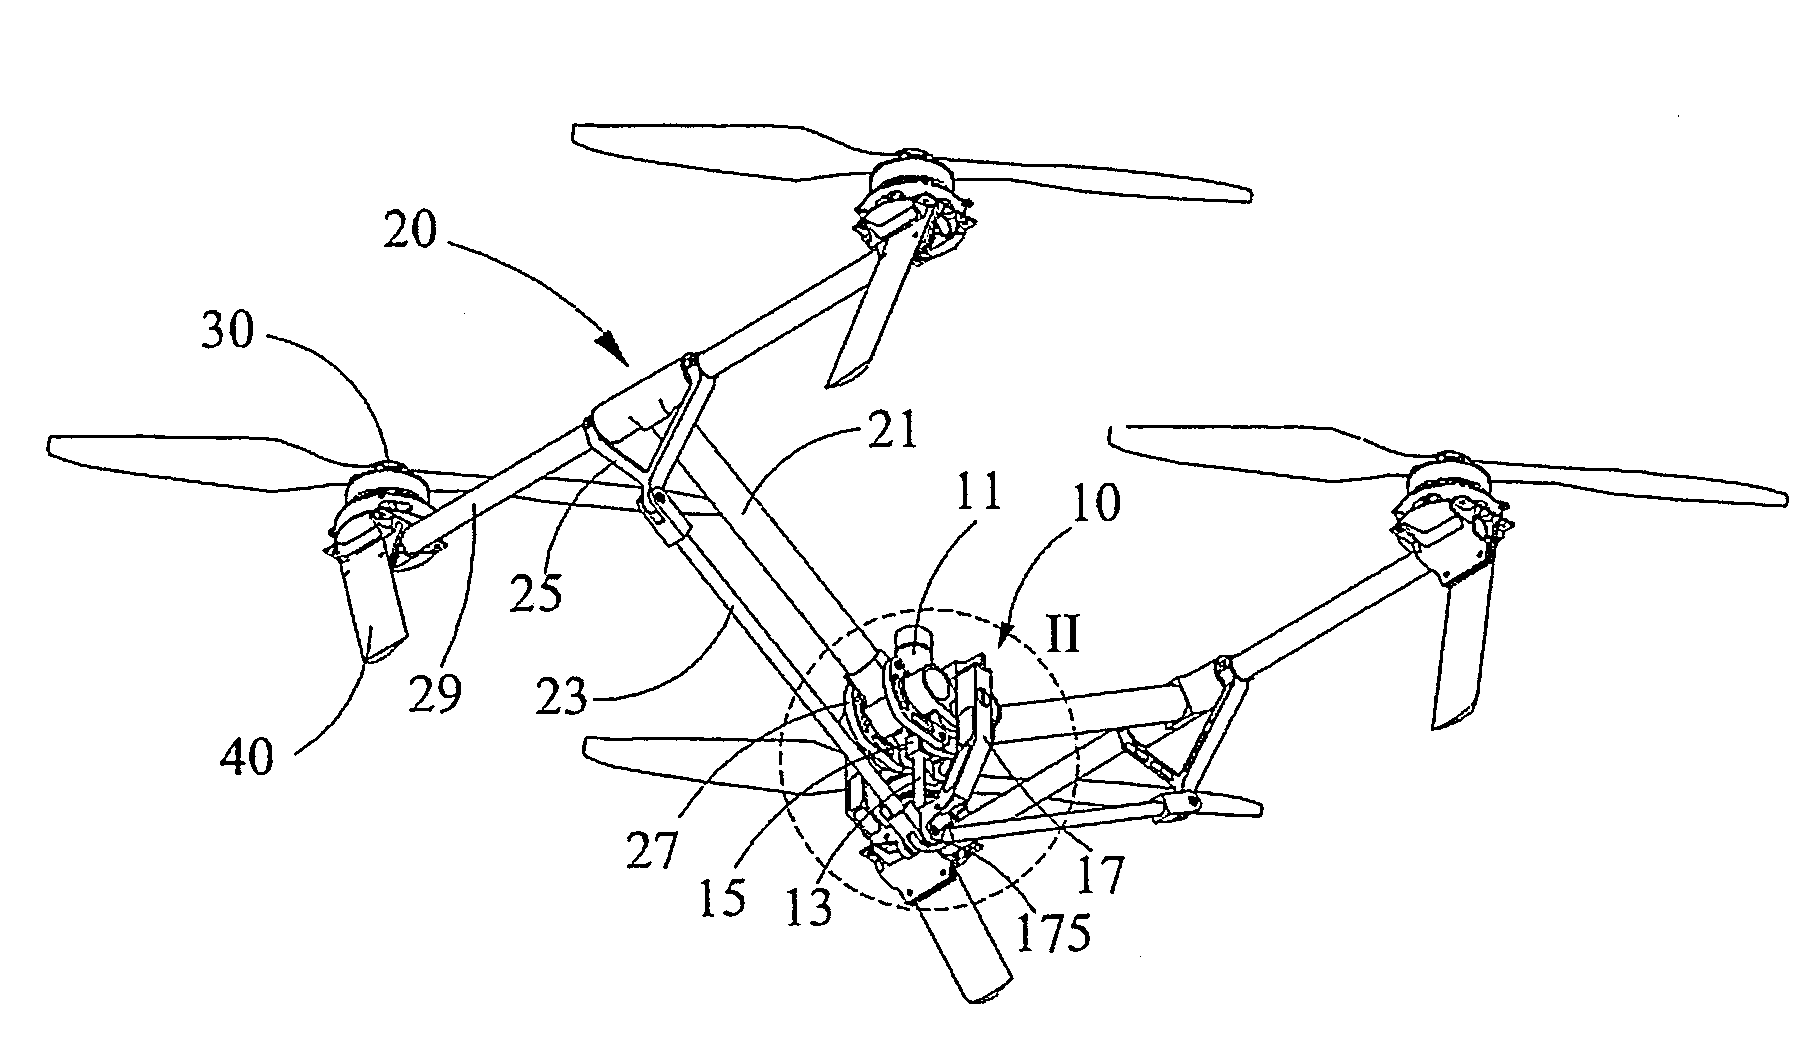
\includegraphics[width=\textwidth]{figs/dji-inspire1}
\caption{Inspire 1 articulated upwards}
\label{fig:inspireup}
\end{subfigure}%
\begin{subfigure}{.5\textwidth}
\centering
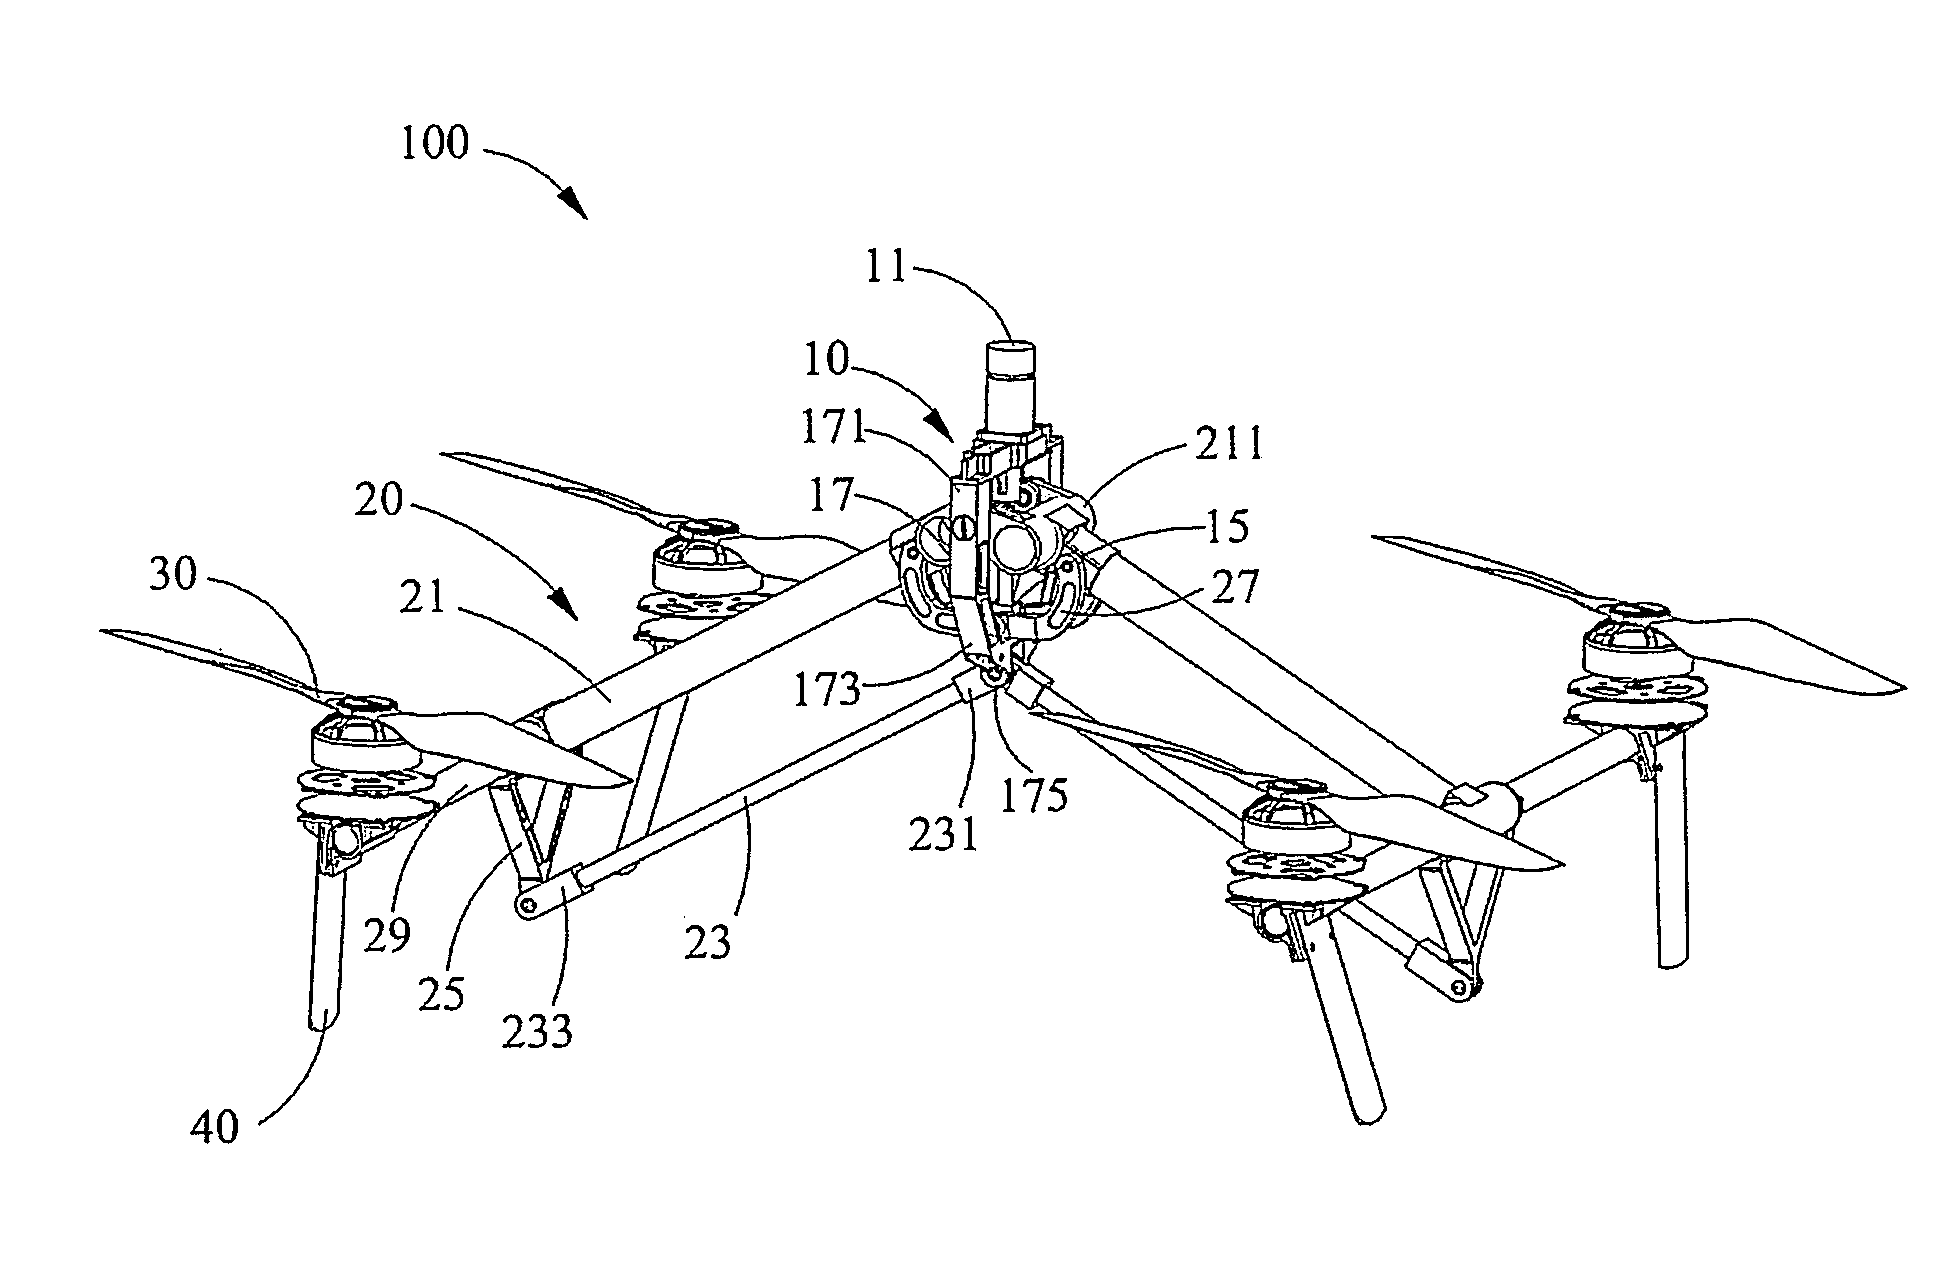
\includegraphics[width=\textwidth]{figs/dji-inspire2}
\caption{Inspire 1 articulated downwards}
\label{fig:inspiredown}
\end{subfigure}
\caption{DJI Inspire 1}
\label{fig:inspire1}
\end{figure}
\par
Another interesting project is that by G.Gres \cite{gres2007} which attempts to use oblique active tilting of a bi-rotor helicopter to induce gyroscopic torques. Whilst the eVader prototype referred to in the paper has dual axis tilting, the actuators are coupled together making the tilt axis 45\textdegree to the bodies' frame. The paper discusses in depth the mechanical system identification aspects of the prototype but, however, gives no insight into attitude control. The author instead discusses the dynamic equations of motion applicable in different flight modes. Whilst the later is irrelevant to quadrotor attitude control, the derivation of induced gyroscopic torque responses as a result of pitching the propellers from their principle plane of rotation is highly pertinent.
\par

\subsection{Notable Control Implementations}
\label{subsec:ch1.lit.notablecontrol}
%----------------------------------------------------

%****************************************************
% END
%****************************************************
